% Provenance (never printed): see sources/outline_sources.md (Year 3:
% ocean dynamics: the Ekman layer derived, the Sverdrup balance, western
% intensification, the abyssal circulation, ocean tides).
% Brief: sources/book5/BRIEFS.md, ch. 21. Curves from
% figdata/bachelor-3/wind_driven_gyre.py and tides.py. Exercise and problem
% values in the Book 5 scratch calculator calc/ch21.py. The basins, winds
% and stations of the exercises and the problem are invented.
\chapter{ديناميكا المحيطات}\label{ch:b3:ocean-dynamics}

عبر مضيق فلوريدا يحمل تيار الخليج نحو الشمال قرابة
\qty{32}{\sverdrup} من الماء، ويزداد حجمه كلّما تبع الساحل
شمالًا حتى قرابة \qty{150}{\sverdrup} قرب \ang{40}~شمالًا. وعلى الجانب الآخر من المحيط نفسه، قبالة البرتغال وشمال
إفريقيا، لا يجري شيء يشبهه نحو الجنوب: فالماء الذي يحمله تيار الخليج
شمالًا يعود نحو خطّ الاستواء على شكل انجراف بطيء واسع عبر آلاف
الكيلومترات من البحر المفتوح. ولكلّ حوض محيطي في نصف الكرة الشمالي
الشكل غير المتماثل نفسه، وتيّاره السريع على جانبه الغربي. أمّا
عدم التماثل فيرجع إلى الرياح، وإلى احتكاك البحر، وإلى حقيقة واحدة
عن الأرض: يتزايد معامل كوريوليس نحو القطب.
% ledger: rapid:transports (31.7 Sv, rounded), stewart:north-atlantic

\begin{recall}
قوة المدّ للقمر والشمس، والمدّ الربيعي والمدّ الميّت، واردة في
كتب الفيزياء. أمّا إجهاد الريح وطبقة إيكمان ونقل إيكمان
وحلزون إيكمان، والصعود والهبوط، والدوّامات المحيطية، وتيارات الحدّ الغربي،
السفيردروب ($\qty{1}{\sverdrup} =
\qty{e6}{m^3/s}$)، والدورة الانقلابية الميريدية،
وتكوين الماء العميق واردة في مجلد السنة الأولى، في فصله عن
دوران المحيطات؛ وهناك يُكتب إجهاد الريح $\vec T$، وهنا
$\vec\tau$. يرد معامل كوريوليس والمستوي $\beta$ ونصف قطر روسبي
والتوازن الجيوستروفي في الفصل~\ref{ch:b3:gfd-foundations}؛
والدوّامية \omterm{def:b3:atmospheric-dynamics:pv}{والدوّامية الكامنة} في الفصل~\ref{ch:b3:atmospheric-dynamics}.
\end{recall}

\section{اشتقاق طبقة إيكمان}\label{sec:b3:ocean-dynamics:ekman}

في مجلد السنة الأولى استُخرج نقل إيكمان من توازن القوى
على الطبقة كلّها، وذُكر حلزون السرعات داخلها. ومع
احتكاك مضطرب بلزوجة دوّامية ثابتة $A_z$، يُستنتج الحلزون
من المعادلات في بضعة أسطر. نكتب السرعة الأفقية عددًا
مركّبًا $W = u + \mathrm iv$، وإجهاد الريح $\tau =
\tau_x + \mathrm i\tau_y$؛ والضرب في $-\mathrm i$ يُدير المتجهة
بمقدار \ang{90} في اتجاه عقارب الساعة، إلى يمينها كما تُرى من الأعلى.

\begin{theorem}[مقطع السرعة لطبقة سطحية مستقرة يحرّكها الريح]\label{thm:b3:ocean-dynamics:ekman}
في محيط مستقر متجانس أفقيًا، بالغ العمق وذي كثافة ثابتة
$\rho$، ولزوجة دوّامية رأسية ثابتة $A_z$، ومعامل كوريوليس
$f > 0$، فإنّ التيار المحرَّك بإجهاد ريح $\tau$ هو
\[
W(z) = W_0\,\mathrm e^{(1+\mathrm i)z/\delta},\qquad
W_0 = \frac{\tau}{\rho\sqrt{fA_z}}\,\mathrm e^{-\mathrm i\pi/4},\qquad
\delta = \sqrt{\frac{2A_z}{f}} ,
\]
حيث $z \le 0$. ويُدار التيار السطحي بمقدار \ang{45} إلى يمين
الإجهاد؛ ومع العمق يدور أكثر نحو اليمين، ويتضاءل وفق $\mathrm
e^{z/\delta}$؛ ونقل الكتلة الكلّي $\int_{-\infty}^0 W\,\mathrm dz =
-\mathrm i\tau/(\rho f)$ عمودي على اتجاه يمين الإجهاد.
\end{theorem}

\begin{proof}
بعيدًا عن السواحل لا يوجد تدرّج أفقي للضغط في الطبقة،
وتوازن قوة كوريوليس الاحتكاك: $-fv = A_z u''$ و$fu =
A_z v''$، إذ تدلّ العلامة $'$ على المشتقّة بالنسبة إلى $z$. نضرب الثانية في
$\mathrm i$ ونجمع فنجد $A_zW'' = \mathrm ifW$. حلولها هي
$\mathrm e^{\pm(1+\mathrm i)z/\delta}$، لأنّ $(1+\mathrm i)^2/\delta^2 =
2\mathrm i/\delta^2 = \mathrm if/A_z$؛ ولا يبقى محدودًا إلا الحدّ ذو الإشارة الموجبة عندما
$z \to -\infty$. وعند السطح يحمل الاحتكاكُ الإجهادَ،
$\rho A_zW'(0) = \tau$، ومنه $W_0 = \tau\delta/(\rho A_z(1+\mathrm i))$.
بما أنّ $\delta/(\sqrt2 A_z) = 1/\sqrt{fA_z}$ و$1/(1+\mathrm i) = \mathrm
e^{-\mathrm i\pi/4}/\sqrt2$، وهذا هو $W_0$ المذكور. ويدور العامل
$\mathrm e^{\mathrm iz/\delta}$ في اتجاه عقارب الساعة كلّما تناقص $z$.
وأخيرًا $\int_{-\infty}^0 W\,\mathrm dz = W_0\delta/(1+\mathrm i) =
\tau\delta^2/(\rho A_z(1+\mathrm i)^2) = \tau\delta^2/(2\mathrm i\rho A_z)
= -\mathrm i\tau/(\rho f)$.
\end{proof}

تستعيد المبرهنة النتيجتين الواردتين في مجلد السنة الأولى: التيار السطحي لإيكمان
عند \ang{45}، والنقل $\tau/(\rho f)$، العمودي على
الإجهاد والمستقلّ عن $A_z$، وهو معامل لا يُعرف جيدًا أبدًا.
وعند العمق $\pi\delta$ يجري التيار عكس التيار السطحي، بعد أن يتضاءل
بعامل $\mathrm e^{-\pi}$ حتى يبلغ \qty{4}{\percent}.

\begin{definition}[عمق إيكمان؛ ضخّ إيكمان]\label{def:b3:ocean-dynamics:ekman-pumping}
\emph{عمق إيكمان}\index{عمق إيكمان} هو $D_E = \pi\delta =
\pi\sqrt{2A_z/f}$، وهو العمق الذي يجري عنده تيار حلزون إيكمان
عكس التيار السطحي؛ وهو يقيس سمك
طبقة إيكمان. \emph{ضخّ إيكمان}\index{ضخّ إيكمان} هو السرعة الرأسية
$w_E$ عند قاعدة طبقة إيكمان التي تفرضها تقارُب أو
تباعُد نقل إيكمان: نحو الأسفل حيث تتقارب النقول،
ونحو الأعلى، ويُسمّى أحيانًا شفط إيكمان، حيث تتباعد.
\end{definition}

\begin{proposition}[ضخّ إيكمان]\label{prop:b3:ocean-dynamics:pumping}
مع انعدام السرعة الرأسية عند سطح البحر، يكون \omterm{def:b3:ocean-dynamics:ekman-pumping}{ضخّ إيكمان}
\[
w_E = \operatorname{curl}_z\frac{\vec\tau}{\rho f}
= \frac{1}{\rho f}\Big(\frac{\partial\tau_y}{\partial x} -
\frac{\partial\tau_x}{\partial y}\Big) + \frac{\beta\tau_x}{\rho f^2} ,
\]
ويُعدّ الاتجاه الصاعد موجبًا.
\end{proposition}

\begin{proof}
النقل الحجمي للطبقة هو $(U_E, V_E) = (\tau_y,
-\tau_x)/(\rho f)$، أي المبرهنة مكتوبةً بالمركّبات. وبتكامل
معادلة الاستمرارية $\partial w/\partial z = -(\partial u/\partial x +
\partial v/\partial y)$ عبر الطبقة، فيصير $w(0) - w_E = -(\partial
U_E/\partial x + \partial V_E/\partial y)$، إذن $w_E = \partial_x(\tau_y/\rho
f) - \partial_y(\tau_x/\rho f)$. وبالنشر باستخدام $\mathrm df/\mathrm dy =
\beta$ نحصل على الصيغة الثانية.
\end{proof}

الريح التي تدور دورانًا إعصاريًّا فوق البحر، وتكون دوّاميّتها موجبة، تسحب
الماء من تحت الطبقة؛ والريح المضادّة للإعصار تدفعه نحو الأسفل. وفوق
المحيطات شبه المدارية تهبّ الرياح التجارية من الشرق على الجانب
المتّجه نحو خط الاستواء، والرياح الغربية من الغرب على الجانب المتّجه نحو القطب. ويتّجه نقل إيكمان
شمالًا تحت الرياح التجارية وجنوبًا تحت الرياح الغربية، فيتقارب
بينهما: يتراكم ماء السطح ويُضخّ نحو الأسفل، كما
في الشكل أدناه. وعلى امتداد ساحل تهبّ فيه الريح
والساحل على يسارها (في نصف الكرة الشمالي)، وفي هذه الحالة
يبتعد النقل عن الشاطئ، والصعود الساحلي المذكور في مجلد السنة الأولى
هو شفط إيكمان مركَّز عند جدار.

\begin{omfigure}
\centering
\begin{tikzpicture}[>=stealth, font=\small, x=1.1cm, y=1cm]
\fill[omThm!7] (-5,0) rectangle (5,-3.6);
\draw[thick] (-5,0) -- (5,0);
\draw[black!45, densely dashed] (-5,-0.9) -- (5,-0.9);
\node[font=\scriptsize, black!60, anchor=north east, inner sep=1pt] at (4.95,-0.95) {طبقة إيكمان};
% winds: west is out of the page, east into the page
\foreach \x in {-4.2,-3.4,-2.6} {\draw (\x,0.55) circle (0.13); \fill (\x,0.55) circle (0.04);}
\foreach \x in {2.6,3.4,4.2} {\draw (\x,0.55) circle (0.13);
  \draw (\x-0.09,0.46) -- (\x+0.09,0.64); \draw (\x-0.09,0.64) -- (\x+0.09,0.46);}
\node[above] at (-3.4,0.75) {الرياح التجارية، من الشرق};
\node[above] at (3.4,0.75) {الرياح الغربية، من الغرب};
% Ekman transports converge
\draw[->, omDef, very thick] (-4.5,-0.45) -- (-1.2,-0.45);
\draw[->, omDef, very thick] (4.5,-0.45) -- (1.2,-0.45);
\node[omDef, font=\scriptsize, fill=omThm!7, inner sep=1pt] at (-2.85,-0.72) {نقل إيكمان};
% pumping
\foreach \x in {-0.6,0,0.6} \draw[->, omThm, thick] (\x,-0.55) -- (\x,-1.55);
\node[omThm, font=\scriptsize, anchor=west] at (0.75,-1.25) {$w_E < 0$};
% squashed column and Sverdrup flow
\draw[thick, black!70] (-0.62,-1.75) rectangle (0.62,-3.1);
\node[font=\scriptsize, black!70, align=center] at (0,-2.42) {العمود\\مضغوط};
\draw[->, omMeth, very thick] (-0.75,-2.42) -- (-3.2,-2.42);
\node[omMeth, font=\scriptsize, align=center, above] at (-2.6,-2.40) {\foreignlanguage{arabic}{جريان سفيردروب،}\\نحو خط الاستواء};
\draw[black!45, densely dashed] (-5,-3.3) -- (5,-3.3);
\node[font=\scriptsize, black!60, anchor=south east, inner sep=1pt] at (4.95,-3.28) {قاع الجريان المدفوع بالرياح};
\node[below, font=\scriptsize] at (-5,-3.6) {جنوب};
\node[below, font=\scriptsize] at (5,-3.6) {شمال};
\end{tikzpicture}

\par\smallskip{\small مقطع شمال--جنوب عبر الدوّامة المحيطية شبه المدارية
من نصف الكرة الشمالي، شرقًا نحو داخل الصفحة. يتقارب نقل إيكمان تحت
الرياح التجارية والرياح الغربية، ويُضخّ الماء نحو الأسفل،
وتتحرّك الأعمدة الواقعة تحتها، المضغوطة، نحو خط الاستواء، حيث $f$ أصغر،
محافظةً على دوّامتها الكامنة.}\label{fig:b3:ocean-dynamics:pumping}
\end{omfigure}

\section{توازن سفيردروب}\label{sec:b3:ocean-dynamics:sverdrup}

تحت طبقة إيكمان يكون المحيط جيوستروفيًّا. وعمودُ الماء الذي
يُضغط بفعل \omterm{def:b3:ocean-dynamics:ekman-pumping}{ضخّ إيكمان}، وللحفاظ على دوّامته الكامنة $f/h$، يجب
أن ينتقل إلى حيث تكون $f$ أصغر: نحو خط الاستواء. وفي عام 1947 جعل \babelsublr{H.~U.} سفيردروب
الحجّةَ كمّيةً لكامل عمق الجريان المدفوع بالرياح.
% ledger: stewart:ekman-layer (Sverdrup 1947)

\begin{theorem}[توازن سفيردروب]\label{thm:b3:ocean-dynamics:sverdrup}
في محيط مستقرّ تكون فيه الحدود غير الخطّية والاحتكاك الجانبي
مهمَلَين، ويكون الداخل جيوستروفيًّا أسفل طبقة إيكمان، وتنعدم
السرعة الشاقولية عند عمقٍ ما $-H$، فإنّ نقل الحجم الشمالي الكلّي لكلّ وحدة عرض
من الجريان المدفوع بالرياح يحقّق \emph{توازن
سفيردروب}\index{توازن سفيردروب}
\[
\beta V = \frac{1}{\rho}\operatorname{curl}_z\vec\tau
= \frac{1}{\rho}\Big(\frac{\partial\tau_y}{\partial x} -
\frac{\partial\tau_x}{\partial y}\Big) .
\]
\end{theorem}

\begin{proof}
في الداخل الجيوستروفي $fv_g = \rho^{-1}\partial p/\partial x$
و$fu_g = -\rho^{-1}\partial p/\partial y$. ومنه $\partial_x(fu_g) +
\partial_y(fv_g) = 0$، أي $f(\partial_xu_g + \partial_yv_g) + \beta
v_g = 0$، ومع معادلة الاستمرارية، $\beta v_g = f\,\partial w/\partial z$.
بالتكامل من $-H$، حيث $w = 0$، حتى قاعدة طبقة إيكمان،
حيث $w = w_E$، نجد $\beta V_g = fw_E$. حسب
\cref{prop:b3:ocean-dynamics:pumping}، $fw_E = \rho^{-1}\operatorname{curl}_z
\vec\tau + \beta\tau_x/(\rho f)$. بإضافة نقل إيكمان $V_E =
-\tau_x/(\rho f)$، مضروبًا في $\beta$، يُلغي الحدّ الأخير:
$\beta(V_g + V_E) = \rho^{-1}\operatorname{curl}_z\vec\tau$.
\end{proof}

يلفت التوازن الانتباه إلى ما لا يحتاجه: لا عمق الجريان،
ولا بنيته الشاقولية، ولا لزوجة \omterm{def:b3:atmospheric-dynamics:eddy}{الاضطراب الدوّامي}، بل فقط
دوّامية الريح و$\beta$. استنتج سفيردروب التوازن من معادلات
الحركة المكاملة حتى عمق انعدام الحركة، واختبره مقابل
المقاطع الهيدروغرافية لسفينتَي الأبحاث \emph{كارنيغي}
و\emph{بوشنل} في شرق المحيط الهادئ الاستوائي، بين \ang{34}~شمالًا
و\ang{10}~جنوبًا، بعمق انعدام الحركة عند \qty{1000}{m}: تطابقت النقول
المحسوبة من الريح مع تلك المحسوبة من حقل الكثافة، حتى حيث كانت
التيارات تجري عكس اتّجاه الريح. وجدت أعمال لاحقة بريّاح أفضل
توافقًا مع عمق انعدام الحركة قرب \qty{500}{m}،
وقياسات متوسّط الإجهاد في المحيط الهادئ الاستوائي عام 1999 وجدت أنّ
الجريان هناك في \omterm{thm:b3:ocean-dynamics:sverdrup}{توازن سفيردروب}. وإثبات أنّ التوازن يصحّ في كلّ مكان
أصعب من افتراضه: تقريبًا كلّ نظرية عن دوران المحيط
تنطلق منه.
% ledger: stewart:sverdrup

خذ الحوض المتخيَّل في مسألة هذا الفصل: بين \ang{20}
و\ang{50}~شمالًا، بعرض \qty{6000}{km}، تحت إجهاد زونالي $\tau_x =
-\tau_0\cos(\pi(\varphi - \ang{20})/\ang{30})$ مع $\tau_0 =
\qty{0.1}{Pa}$، شرقيًّا عند \ang{20}~شمالًا، غربيًّا عند \ang{50}~شمالًا، صفرًا عند
\ang{35}~شمالًا. وعلى معظم الحوض تكون دوّامية الإجهاد سالبة:
يُضخّ الماء إلى الأسفل بمقدار نحو \qty{35}{m} في السنة عند \ang{35}~شمالًا، ويجري
الداخل جنوبًا، بنقل \qty{4.9}{m^2/s} لكلّ متر من العرض عند \ang{35}~شمالًا،
\qty{29.4}{\sverdrup} عبر الحوض. وإذا حُسب من الرياح المرصودة،
يبلغ نقل سفيردروب في الدوّامة المحيطية شبه المدارية لشمال الأطلسي نحو
\qty{30}{\sverdrup} قرب \ang{28}~شمالًا.
% ledger: stewart:north-atlantic (computed in figdata/bachelor-3/wind_driven_gyre.py)

\begin{omfigure}
\begin{tikzpicture}
\begin{groupplot}[group style={group size=3 by 1, horizontal sep=0.45cm, yticklabels at=edge left},
  width=0.37\linewidth, height=0.46\linewidth, ymin=20, ymax=50, ytick={20,25,30,35,40,45,50},
  tick label style={font=\scriptsize}, label style={font=\small}, title style={font=\small}]
\nextgroupplot[xlabel={إجهاد الريح $\tau_x$ \babelsublr{(\unit{Pa})}}, ylabel={خط العرض (\unit{\degree} شمالًا)},
  xmin=-0.12, xmax=0.12, xtick={-0.1,0,0.1}, title={إجهاد الريح},
  scaled x ticks=false, xticklabel style={/pgf/number format/fixed}]
% computed in figdata/bachelor-3/wind_driven_gyre.py
\addplot[black!50, thin] coordinates {(0,20) (0,50)};
\addplot[omThm, thick] table[x=tau, y=lat] {figdata/out/bachelor-3-wind_driven_gyre-merid.dat};
\nextgroupplot[xlabel={ضخّ إيكمان $w_E$ \babelsublr{(\unit{m/yr})}}, xmin=-45, xmax=12, xtick={-40,-20,0},
  title={ضخّ إيكمان}]
\addplot[black!50, thin] coordinates {(0,20) (0,50)};
\addplot[omDef, thick] table[x=wE, y=lat] {figdata/out/bachelor-3-wind_driven_gyre-merid.dat};
\nextgroupplot[xlabel={النقل \babelsublr{(\unit{\sverdrup})}}, xmin=-32, xmax=10, xtick={-30,-20,-10,0,10},
  title={سفيردروب}]
\addplot[black!50, thin] coordinates {(0,20) (0,50)};
\addplot[omMeth, thick] table[x=Vtot, y=lat] {figdata/out/bachelor-3-wind_driven_gyre-merid.dat};
\end{groupplot}
\end{tikzpicture}

\par\smallskip{\small الحوض المتخيَّل في مسألة هذا الفصل، من \ang{20} إلى
\ang{50}~شمالًا، بعرض \qty{6000}{km}. يسارًا، إجهاد الريح الزونالي، موجبًا شرقًا.
وسطًا، \omterm{def:b3:ocean-dynamics:ekman-pumping}{ضخّ إيكمان}، موجبًا نحو الأعلى: يُدفع الماء إلى الأسفل
جنوبَ \ang{47}~شمالًا، وأقوى ما يكون في الجنوب حيث $f$ صغير،
ويُسحب إلى الأعلى شمالَ ذلك. يمينًا، نقل سفيردروب الكلّي المتّجه شمالًا عبر الحوض:
يتّجه الداخل جنوبًا، \qty{29.4}{\sverdrup} عند \ang{35}~شمالًا، باستثناء
شريط رفيع عند الحافة الشمالية، حيث تتغيّر إشارة دوّامية الإجهاد.}\label{fig:b3:ocean-dynamics:sverdrup}
\end{omfigure}
% ledger: earth:Rmean, geod5:grs80-defining

يحدّد نقل سفيردروب قيمة $V$ عند كلّ نقطة، لكنّ دالّة التيار
تحتاج إلى شرط حدّي، والجدار الزوالي لا يتّسع إلا لشرط واحد. فإذا
لا يُحقِّق الداخل تدفّقًا عبر الجدار الشرقي، فإنّ التدفّق الجنوبي
لا يجد مخرجًا عند الجدار الغربي؛ فتُعاد الكتلة بتيار
لا تستطيع معادلات سفيردروب، من دون احتكاك، أن تصفه.

\section{الاشتداد الغربي}\label{sec:b3:ocean-dynamics:western}

في عام 1948 أضاف ستوميل أبسط احتكاك إلى أبسط محيط، ووجد
أنّ التدفّق الراجع يتكدّس عند الجدار الغربي، كما في شكل
مجلد السنة الأولى لدوّامته. ولم يجده إلّا مع معامل كوريوليس
الذي يتزايد نحو الشمال؛ فمن دون دوران، أو مع معامل منتظم،
كانت دوّامته متماثلة.
% ledger: stewart:stommel, stommel:1948

\begin{definition}[الاشتداد الغربي؛ نموذج ستوميل؛ طبقة مونك الحدّية]\label{def:b3:ocean-dynamics:western-intensification}
\emph{الاشتداد الغربي}\index{الاشتداد الغربي} هو
تكدّس التدفّق الراجع لدوّامة محيطية محرَّكة بالرياح في تيار ضيّق وسريع
يجري بمحاذاة الجانب الغربي للحوض. أمّا \emph{نموذج ستوميل}\index{نموذج ستوميل}
فهو محيط متجانس ذو عمق ثابت في حوض مستطيل،
يحرّكه إجهاد ريح زونالي، ويُكبح باحتكاك القاع
المتناسب مع السرعة المتكاملة عبر العمق، بمعدّل $r$؛
ودالّة التيار للنقل $\psi$ ($U = -\partial\psi/\partial y$، $V =
\partial\psi/\partial x$) تخضع للمعادلة الآتية
\[
r\nabla^2\psi + \beta\frac{\partial\psi}{\partial x} =
\frac{1}{\rho}\operatorname{curl}_z\vec\tau ,\qquad \psi = 0 \text{ على الجدران.}
\]
أمّا \emph{طبقة مونك الحدّية}\index{طبقة مونك الحدّية} فهي الطبقة الحدّية الغربية
للدوّامة نفسها حين تحلّ لزوجة دوّامية جانبية $A_H$
محلّ احتكاك القاع، ومقياس عرضها هو $\delta_M =
(A_H/\beta)^{1/3}$.
\end{definition}

المعادلة هي \omterm{thm:b3:ocean-dynamics:sverdrup}{توازن سفيردروب} مع إضافة دوّامة احتكاك القاع،
متكاملةً عبر العمق: $\beta V = \rho^{-1}\operatorname{curl}_z
\vec\tau - r\zeta_T$، حيث $\zeta_T = \nabla^2\psi$ هي دوّامية
النقل.

\begin{theorem}[الطبقة الحدّية الغربية لدوّامة ستوميل]\label{thm:b3:ocean-dynamics:stommel}
في حوض $0 \le x \le X$، و$0 \le y \le L$، مع $\tau_x = -\tau_0
\cos(\pi y/L)$، و$\delta_S = r/\beta \ll X$، فإنّ دالّة تيار ستوميل
هي، إلى الرتبة الأولى في $\delta_S/X$،
\[
\psi = A\sin\frac{\pi y}{L}\Big[(X - x) - X\mathrm e^{-x/\delta_S}\Big],
\qquad A = \frac{\pi\tau_0}{\rho\beta L} .
\]
يحمل الداخل $AX\sin(\pi y/L)$ جنوبًا، وتُعيد طبقة حدّية بعرض
$\delta_S$ مقابل الجدار الغربي تعيده شمالًا؛ ولا يمكن أن
توجد طبقة حدّية مقابل الجدار الشرقي.
\end{theorem}

\begin{proof}
دوّامة الإجهاد هي $-\partial\tau_x/\partial y = -(\pi\tau_0/L)\sin(\pi
y/L)$. وعلى عرض الحوض يكون حدّ الاحتكاك أصغر من حدّ
$\beta$ بمقدار $\delta_S/X$؛ وبإسقاطه يبقى \omterm{thm:b3:ocean-dynamics:sverdrup}{توازن سفيردروب}،
$\beta\,\partial\psi/\partial x = -(\pi\tau_0/\rho L)\sin(\pi y/L)$، الذي يتلاشى حلّه عند
$x = X$ هو $\psi_I = A\sin(\pi y/L)(X - x)$. ولا يتلاشى
عند $x = 0$. وقرب الجدار يتغيّر $\psi$ بسرعة في $x$، فتُختزل
المعادلة إلى $r\,\partial^2\psi/\partial x^2 + \beta\,\partial\psi/
\partial x = 0$ لأجل التصحيح، وحلّاه ثابتٌ
و$\mathrm e^{-x/\delta_S}$. ويتناقص هذا الحلّ شرقًا، مبتعدًا عن الجدار الغربي:
إضافة $-AX\sin(\pi y/L)\,\mathrm e^{-x/\delta_S}$ تجعل $\psi = 0$
عند $x = 0$ ولا تغيّر شيئًا في الداخل. وعند الجدار الشرقي يلزم أن يتناقص
التصحيح غربًا، مبتعدًا عن $x = X$،
و$\mathrm e^{-x/\delta_S}$ يتزايد غربًا: لا توجد طبقة كهذه، فيلزم أن
يلتقي الداخل بالجدار الشرقي من تلقاء نفسه، كما يفعل $\psi_I$.
والنقل الشمالي بين الجدار والنقطة التي تتغيّر عندها إشارة $V$
هو $\psi$ هناك، قريبًا من $AX\sin(\pi y/L)$.
\end{proof}

يأتي الجواب نفسه من الدوّامية. فوق الداخل تمنح الرياحُ كلَّ عمود
دوّامية سالبة، ويدفع العمود ثمن ذلك بالتحرّك جنوبًا،
نحو $f$ أصغر. وفي طريق العودة شمالًا يكتسب \omterm{def:b3:atmospheric-dynamics:vorticity-kinds}{الدوّامية الكوكبية}،
ويجب أن يفقدها، ولا يفعل ذلك إلّا الاحتكاك. وفي تيار متجه شمالًا تتناقص سرعته شرقًا
انطلاقًا من قرب الجدار الغربي، فإنّ $\partial
v/\partial x < 0$ على معظم عرضه: دوّامية التيار سالبة، والاحتكاك يعمل ضدّها،
فيوفّر الدوّامية الموجبة التي تحتاجها الأعمدة. أمّا تيار متجه شمالًا
عند جدار شرقي فستكون دوّاميته موجبة، وكان
الاحتكاك سيُزيل الإشارة الخاطئة.

\begin{omfigure}
\begin{tikzpicture}
\begin{groupplot}[group style={group size=2 by 1, horizontal sep=1.7cm},
  width=0.48\linewidth, height=0.42\linewidth, xmin=0, xmax=400,
  xlabel={المسافة من الجدار الغربي \babelsublr{(\unit{km})}},
  tick label style={font=\scriptsize}, label style={font=\small},
  legend style={font=\scriptsize, draw=none, fill=none}]
\nextgroupplot[ylabel={السرعة $V$ \babelsublr{(\unit{m^2/s})}}, ymin=-80, ymax=600, legend pos=north east,
  legend cell align=left]
% computed in figdata/bachelor-3/wind_driven_gyre.py
\addplot[omThm, thick] table[x=x, y=vS] {figdata/out/bachelor-3-wind_driven_gyre-bl.dat};
\addlegendentry{\foreignlanguage{arabic}{ستوميل، \mbox{\textdir TLT $\delta_S = \qty{53}{km}$}}}
\addplot[omDef, thick] table[x=x, y=vM] {figdata/out/bachelor-3-wind_driven_gyre-bl.dat};
\addlegendentry{\foreignlanguage{arabic}{مونك، \mbox{\textdir TLT $\delta_M = \qty{64}{km}$}}}
\addplot[black!50, thin, forget plot] coordinates {(0,0) (400,0)};
\nextgroupplot[ylabel={النقل من الجدار \babelsublr{(\unit{\sverdrup})}}, ymin=0, ymax=36,
  legend pos=south east, legend cell align=left]
\addplot[omThm, thick] table[x=x, y=cS] {figdata/out/bachelor-3-wind_driven_gyre-bl.dat};
\addlegendentry{ستوميل}
\addplot[omDef, thick] table[x=x, y=cM] {figdata/out/bachelor-3-wind_driven_gyre-bl.dat};
\addlegendentry{مونك}
\addplot[black!60, densely dashed] coordinates {(0,29.4) (400,29.4)};
\addlegendentry{\foreignlanguage{arabic}{الداخل، \mbox{\textdir TLT \qty{29.4}{\sverdrup}}}}
\end{groupplot}
\end{tikzpicture}

\par\smallskip{\small الطبقة الحدّية الغربية عند منتصف
الحوض المتخيَّل في المسألة (\ang{35}~شمالًا، عرضه \qty{6000}{km}). يسارًا، النقل
نحو الشمال لكلّ وحدة عرض: طبقة ستوميل، مع احتكاك قاعي
$r = \qty{e-6}{s^{-1}}$، يتناقص أُسيًّا من الجدار؛ وطبقة مونك، مع
$A_H = \qty{5e3}{m^2/s}$ وبلا انزلاق عند الجدار، ترتفع من الصفر وتبلغ ذروتها
على بُعد نحو \qty{80}{km} منه، ويليها تيار مضاد ضعيف متّجه جنوبًا.
يمينًا، النقل بين الجدار وكلّ مسافة، في مقابل
\qty{29.4}{\sverdrup} الذي يحمله الداخل جنوبًا: تجمع طبقة ستوميل
\qty{27.9}{\sverdrup} قبل أن يتحوّل تدفّقها جنوبًا، ويجمع تيار مونك
\qty{33.0}{\sverdrup} قبل تيّاره المضاد.}\label{fig:b3:ocean-dynamics:boundary}
\end{omfigure}
% ledger: stewart:munk

مع $r = \qty{e-6}{s^{-1}}$ عند \ang{35}~شمالًا، و$\delta_S = \qty{53}{km}$،
ويشغل التدفّق الشمالي أوّل \qty{250}{km} من الجدار. وفي عام 1950
و.~ه.~مونك استبدل الاحتكاك القاعي بلزوجة \omterm{def:b3:atmospheric-dynamics:eddy}{الاضطراب الدوّامي} الجانبية $A_H$،
الذي يؤثّر في القصّ داخل التيار؛ فتكتسب المعادلة حدًّا
$A_H\nabla^4\psi$، وقرب الجدار الغربي يصبح التصحيح
$\mathrm e^{-x/2\delta_M}$ مضروبًا في تذبذب، $\cos(\sqrt3x/2\delta_M)$
و$\sin(\sqrt3x/2\delta_M)$. ومع $A_H = \qty{5e3}{m^2/s}$ يكون التيار الشمالي
عرضه نحو \qty{225}{km} (في حوض الشكل، \qty{233}{km})،
يليه تيار مضاد ضعيف، وهو شكل قريب من تيار الخليج
وكوروشيو. كما في طبقة ستوميل، لا يتعلّق نقل التيار
بالاحتكاك، بل بدوّامية إجهاد الريح وعرض
الحوض و$\beta$. ومن رياح عصره حسب مونك
\qty{36}{\sverdrup} لتيار الخليج، و\qty{39}{\sverdrup} لتيار
كوروشيو، نحو نصف قيم النقل المقاسة آنذاك؛ ومع معامل
السحب الأفضل ومتوسّطات أدقّ للإجهاد، وُجد \qty{32}{\sverdrup}
لتيار الخليج عام 1978. ويُقاس في معظمه بكابل بحري،
ظلّ تيار الخليج في مضيق فلوريدا يحمل \qty{31.7}{\sverdrup} على
المتوسّط منذ عام 2004. ويزداد تدفّقه باتجاه المصبّ حتى نحو \qty{150}{\sverdrup} قرب
\ang{40}~شمالًا، وقبالة رأس هاتيراس يحدث تدوير قوي
لا تتضمّنه النظرية الخطّية، فيُفسد التوافق.
% ledger: stewart:munk, rapid:transports, stewart:north-atlantic

\section{الدوران الأعماقي}\label{sec:b3:ocean-dynamics:abyssal}

يُملأ المحيط العميق من أماكن قليلة. وفي مجلد السنة الأولى، يتكوّن الماء العميق
حيث يُبرَّد الماء السطحي ويُجعل كثيفًا في أقصى شمال
الأطلسي وحول القارة القطبية الجنوبية، وينتشر عبر الأحواض بوصفه ماء الأطلسي الشمالي
العميق وماء القاع القطبي الجنوبي. بين عامَي 1958 و1960
ه.~ستوميل وأ.~ب.~آرونز وأ.~ج.~فالر تساءلوا كيف ينتشر، مستعينين
بالحجّة الدوّامية نفسها التي استعملها سفيردروب.

\begin{definition}[نموذج ستوميل--آرونز]\label{def:b3:ocean-dynamics:abyssal}
\emph{نموذج ستوميل--آرونز}\index{نموذج ستوميل--آرونز} للدوران الأعماقي يفترض أنّ
الماء العميق يُغذّى بالحمل عند عدد قليل من
المنابع عالية العرض، وأنّه يعود إلى المحيط العلوي عبر صعود بطيء منتظم
$W_0$ عبر قاعدة المنحدر الحراري، يوازنه خلط الحرارة نحو الأسفل، وأنّ
التدفّق الداخلي جيوستروفي ويحفظ
\omterm{def:b3:atmospheric-dynamics:pv}{الدوّامية الكامنة}. وتُغلق الدورة بتيارات الحدّ الغربي
العميقة.
\end{definition}

\begin{proposition}[التدفّق الداخلي في الأعماق نحو القطبين]\label{prop:b3:ocean-dynamics:abyssal}
في \omterm{def:b3:ocean-dynamics:abyssal}{نموذج ستوميل--آرونز}، فوق قاع مستوٍ، يكون النقل المكامَل على العمق
نحو الشمال للداخل الأعماقي يُعطى بالعلاقة
\[
V = \frac{f}{\beta}W_0 = a\tan\varphi\,W_0 ,
\]
متّجهًا نحو القطبين في نصفي الكرة كليهما عندما $W_0 > 0$.
\end{proposition}

\begin{proof}
في الداخل الجيوستروفي، $\beta v = f\,\partial w/\partial z$، كما في
برهان \omterm{thm:b3:ocean-dynamics:sverdrup}{توازن سفيردروب}. بالتكامل من القاع المستوي، حيث
$w = 0$، حتّى أعلى الطبقة الأعماقية حيث $w = W_0$، نجد $\beta V =
fW_0$، و$f/\beta = 2\Omega\sin\varphi\,a/(2\Omega\cos\varphi) =
a\tan\varphi$. وفي نصف الكرة الجنوبي $\tan\varphi < 0$: يكون التدفّق
جنوبًا، وهو متّجه نحو القطب أيضًا.
\end{proof}

النتيجة مخالفة للحدس: يتدفّق الداخل الأعماقي نحو
المنابع، لا مبتعدًا عنها. أجرى ستوميل وآرونز تجارب بالأحواض الدوّارة
ليقتنعا بها. يسير الماء القادم من المنابع
على امتداد الجدران الغربية، في تيارات الحدّ الغربي العميقة التي تغذّي
الداخل في أثناء مسيرها. وفي قطاع من المحيط بين خطّ الاستواء والقطب
يقع فيه المنبع كلّه $S_0$ قرب القطب، ويحمل تيار الحدّ الغربي
$2S_0\sin\varphi$ نحو خطّ الاستواء، أي ضعف المنبع عند القطب
ولا شيء عند خطّ الاستواء: الفائض عن $S_0$ هو ماء معاد تدويره
من الداخل. يجعل النموذج الدوران العميق مدفوعًا بالخلط
لا بالهبوط: لو غاب الصعود لاقتصر الحمل على ملء
الأعماق ببركة راكدة من الماء البارد. وتتراوح أزمنة عبورها بين
بضعة قرون قرب المنابع إلى ما يقارب ألف سنة في شمال
الهادئ. وفوق قاع المحيط الفعلي تقسّم الظهرات الأحواض، ويكون الخلط
قويًّا فوق التضاريس الخشنة، والتدفّق العميق نطاقيّ أكثر بكثير من
تدفّق النموذج. وأبقى تنبّؤاته هو تيار الحدّ الغربي العميق: ففي
شمال الأطلسي يعود نحو \qty{14}{\sverdrup} من الماء
عند \qty{2}{\celsius} جنوبًا، بينما يحمل تيار الخليج الماء الدافئ
شمالًا.
% ledger: stewart:stommel-arons, stewart:deep-circulation, stewart:heat-conveyor

\begin{omfigure}
\centering
\begin{tikzpicture}[>=stealth, font=\small, scale=0.95]
\fill[omThm!7] (0,0) -- (7,0) -- (4.2,5) -- (2.8,5) -- cycle;
\draw[thick] (0,0) -- (2.8,5) -- (4.2,5) -- (7,0);
\draw[black!45, densely dashed] (0,0) -- (7,0);
\node[below, font=\scriptsize] at (3.5,0) {خط الاستواء};
\node[above, font=\scriptsize] at (3.5,5) {نحو القطب};
\fill[omThm] (3.05,4.6) circle (0.17);
\node[font=\scriptsize, anchor=west, inner sep=1pt] at (3.22,4.6) {$S_0$};
% western boundary current
\draw[->, omThm, very thick] (2.75,4.35) -- (0.35,0.25);
\node[omThm, font=\scriptsize, rotate=60.8, inner sep=1pt] at (0.85,2.45) {التيار الحدّي الغربي العميق};
% interior poleward flow
\foreach \x/\y in {2.6/0.7, 3.8/0.7, 5.0/0.7, 3.1/1.7, 4.3/1.7, 3.6/2.7, 4.6/2.7} {
  \draw[->, omMeth, thick] (\x,\y) -- ++(0.15,0.65);}
% upwelling dots
\foreach \x/\y in {2.2/1.25, 3.4/1.25, 4.6/1.25, 5.6/1.25, 2.7/2.2, 3.9/2.2, 5.0/2.2, 3.3/3.2, 4.3/3.2, 3.8/3.9} {
  \draw[omDef] (\x,\y) circle (0.09); \fill[omDef] (\x,\y) circle (0.03);}
\node[omMeth, font=\scriptsize, align=left, anchor=west] at (6.45,2.6) {تدفّق داخلي\\نحو القطب};
\node[omDef, font=\scriptsize, align=left, anchor=west] at (6.6,1.5) {\foreignlanguage{arabic}{الصعود $W_0$}};
\end{tikzpicture}

\par\smallskip{\small يبيّن الشكل دوران ستوميل--آرونز في الأعماق، في قطاع
من محيط نصف الكرة الشمالي، كما يُرى من الأعلى. يغوص الماء العميق عند
المصدر $S_0$ قرب القطب، ويجري نحو خط الاستواء في تيار حدّي غربي عميق،
ويتسرّب إلى داخل يتحرّك نحو القطب،
ويصعد ببطء في كل مكان عبر المنحدر الحراري (النقاط تمثّل
الصعود نحو القارئ).}\label{fig:b3:ocean-dynamics:stommel-arons}
\end{omfigure}

المنطقة الداخلية للنموذج، كما عند سفيردروب، جيوستروفية، والتيارات
الجيوستروفية للبحر العميق تُقاس بالطريقة التي قاس بها سفيردروب
تياراته: من الكثافة.

\begin{definition}[الطريقة الديناميكية]\label{def:b3:ocean-dynamics:dynamic-height}
\emph{الطريقة الديناميكية}\index{الطريقة الديناميكية} تحسب التيار الجيوستروفي
بين محطتين هيدروغرافيتين من الكثافة المقاسة في كلتيهما،
بالنسبة إلى مستوى ضغط مرجعي يُفترض عنده أن
التيار معدوم أو معلوم. تُقسَم المسافة الجهدية بين سطحي ضغط،
أي $\int\alpha\,\mathrm dp$ حيث $\alpha = 1/\rho$ هو الحجم النوعي،
إلى جزء قياسي متساوٍ في المحطتين،
و\emph{الشذوذ الجهدي الأرضي} $\Delta\Phi$؛ ويكون التيار عند السطح العلوي،
عموديًا على الخط الواصل بين المحطتين $A$ و$B$، والمسافة بينهما $L$
هو
\[
v = \frac{\Delta\Phi_B - \Delta\Phi_A}{fL} .
\]
\end{definition}

لماذا لا يُقاس الضغط مباشرةً، كما يفعل علماء الأرصاد الجوية؟ يحتاج تيار جيوستروفي
مقداره \qty{10}{cm/s} عند \ang{30} إلى تدرّج ضغط مقداره \qty{7.5e-3}{Pa/m}،
أي \qty{750}{Pa} عبر \qty{100}{km}، وهو وزن \qty{7.4}{cm} من ماء البحر.
ولا يمكن ضبط أي مقياس ضغط على قاع البحر بهذه الدقة.
أما الكثافة، المحسوبة بدقة بضعة أجزاء في المليون، فتعطي
ميل سطح ضغط بالنسبة إلى آخر. يقع الماء الأخفّ والأدفأ على يمين التيار،
عند النظر في اتجاهه، في نصف الكرة الشمالي.
وعبر تيار الخليج تتغيّر أعماق أسطح الكثافة الثابتة
بأكثر من \qty{1}{km} عبر \qty{100}{km}.
% ledger: stewart:dynamic-method

\begin{method}[التيار الجيوستروفي من محطتين]\label{met:b3:ocean-dynamics:dynamic}
\begin{enumerate}
\item عند كل محطة، احسب شذوذ الحجم النوعي $\delta =
  \alpha(S, T, p) - \alpha(35, 0, p)$ من الملوحة المقاسة،
  ودرجة الحرارة والضغط.
\item أجرِ التكامل من مستوى الضغط المرجعي حتى كل ضغط $p$:
  $\Delta\Phi(p) = \int_p^{p_{\text{مرجع}}}\delta\,\mathrm dp$.
\item عند كل ضغط، يكون $v(p) = (\Delta\Phi_B - \Delta\Phi_A)/(fL)$
  هو التيار بالنسبة إلى المستوى المرجعي، موجبًا عندما تكون المحطة $B$
  على اليمين.
\item أضِف تيار المستوى المرجعي إن كان معلومًا، من عوّامة
  تنجرف عنده، أو من ميل سطح البحر المقاس بالأقمار الصناعية.
\end{enumerate}
\end{method}

\begin{inthefield}[مصفوفة من العوّامات]
\begin{minipage}[t]{0.52\linewidth}\vspace{0pt}
\begin{dated}{2024}
تنجرف نحو أربعة آلاف عوّامة من نوع Argo عبر المحيط العالمي. تُنزَل
من جانب السفينة فتغوص عوّامة إلى نحو \qty{1000}{m} وتنجرف هناك نحو تسعة أيام؛
ثم تغوص إلى \qty{2000}{m} وتصعد إلى السطح، فتقيس الناقلية والحرارة
والضغط في أثناء الصعود، ويبدأ الدورة من جديد كل نحو عشرة أيام؛
وتصل عوّامات أرغو العميقة في قياساتها إلى
\qty{6000}{m}. وفي يوليو 2024 جمعت المصفوفة قياسها رقم ثلاثة ملايين.
ومن هذه القياسات يحسب علماء المحيطات \omterm{def:b3:ocean-dynamics:dynamic-height}{الشذوذات الجهدية} الأرضية للطريقة
الديناميكية عند كل عوّامة، والإزاحة الذاتية للعوّامة بين صعودين متتاليين
تعطي متوسط التيار عند عمق توقّفها، وهي السرعة المرجعية التي اضطرّ سفيردروب
إلى افتراضها، وقد أصبحت تُقاس الآن.
\end{dated}
\end{minipage}\hfill
\begin{minipage}[t]{0.44\linewidth}\vspace{0pt}
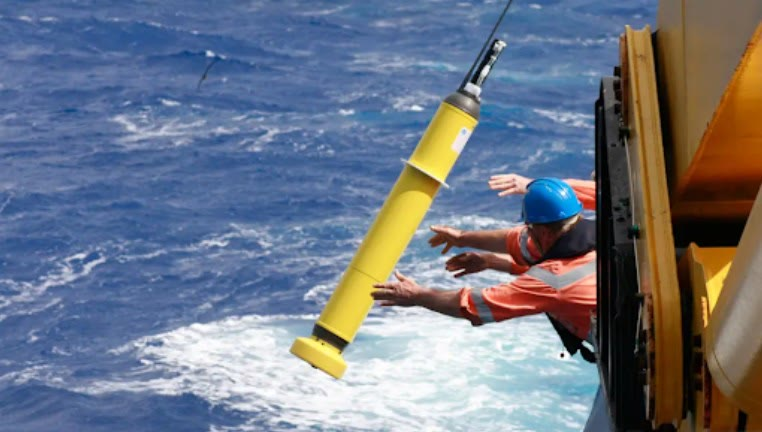
\includegraphics[width=\linewidth]{images/book5/b3-argo-deploy.jpg}

{\scriptsize عوّامة Argo تُنزَل من جانب سفينة بحث علمي (NOAA
\babelsublr{Global Ocean Monitoring and Observing Program}، ملك عام).}
\end{minipage}
\end{inthefield}
% ledger: argo:fleet, noaa:argo-25, photo:b3-argo-deploy

\section{المدّ في المحيطات}\label{sec:b3:ocean-dynamics:tides}

يحدث المدّ مرتين كل يوم، ويتأخّر كل يوم بما يقلّ قليلًا عن ساعة، فيرتفع البحر
وينخفض. تشرح كتب الفيزياء قوة المدّ: فجذب القمر
أقوى في الجانب القريب من الأرض منه في مركزها، وأضعف في
الجانب البعيد، فيُسحب الماء بالنسبة إلى المركز على امتداد
الخط الواصل إلى القمر على الجانبين معًا.

\begin{definition}[مدّ التوازن؛ المكوّن المدّي]\label{def:b3:ocean-dynamics:tides}
\emph{مدّ التوازن}\index{مدّ التوازن} هو الشكل الذي تتّخذه
سطح محيط يغطي الأرض كلها لو تبع جهد توليد المدّ
لحظيًا دون قصور ذاتي. \emph{المكوّن
المدّي}\index{المكوّن المدّي} هو أحد الحدود التوافقية، ولكلّ منها
تردّد ثابت تحدّده حركات القمر والشمس، وسعة وطور يُحسبان
عند كل مكان، ويجتمع مجموعها ليكوّن المدّ؛ وتُسمّى
بحرف وعدد الدورات في اليوم، مثل M$_2$، المكوّن
القمري نصف اليومي الرئيسي.
\end{definition}

\begin{theorem}[مدّ التوازن للقمر]\label{thm:b3:ocean-dynamics:equilibrium-tide}
بالنسبة إلى القمر، ذي الكتلة $M$ على بُعد $d$ من مركز الأرض، ذات
الكتلة $M_E$ ونصف القطر $a$، فإنّ \omterm{def:b3:ocean-dynamics:tides}{مدّ التوازن} عند زاوية $\theta$ من
النقطة الواقعة تحت القمر يساوي
\[
\eta = K\,\frac{3\cos^2\theta - 1}{2},\qquad
K = \frac{M}{M_E}\Big(\frac{a}{d}\Big)^3 a .
\]
\end{theorem}

\begin{proof}
جهد القمر عند نقطة تبعد $a$ عن مركز الأرض
وتصنع زاوية $\theta$ هو $-GM/s$، مع $s^2 = d^2 - 2ad\cos\theta +
a^2$. نشرّ بدلالة $a/d$، فنجد $1/s = (1/d)[1 + (a/d)\cos\theta + (a/d)^2
(3\cos^2\theta - 1)/2 + \cdots]$. الحدّ الأول ثابت، والحدّ الثاني
مجال منتظم، وهو الذي يُسرّع الأرض كلها في مدارها
حول مركز الكتلة المشترك، ولا أثر له بالنسبة إلى الأرض.
ما يبقى هو جهد توليد المدّ $\Phi_T = -(GMa^2/d^3)(3
\cos^2\theta - 1)/2$. في حالة التوازن يكون سطح البحر سطحًا لجهد كلّي
ثابت، $g\eta + \Phi_T = C$، حيث $g = GM_E/a^2$، ومنه
$\eta = (M/M_E)(a^4/d^3)(3\cos^2\theta - 1)/2 + C/g$. ومتوسط
$3\cos^2\theta - 1$ على الكرة معدوم؛ ولأنّ حجم الماء
ثابت، فإنّ $C = 0$.
\end{proof}

مع نسبة الكتلة $0.0123$، و$d = \qty{384400}{km}$ و$a =
\qty{6371}{km}$، و$K = \qty{0.357}{m}$، يقف البحر على ارتفاع \qty{0.36}{m}
تحت القمر وفي الجهة المقابلة، وينخفض \qty{0.18}{m} على
الدائرة العظمى الواقعة بينهما، فيكون المدى \qty{0.54}{m}. عند خط العرض $\varphi$،
والقمر في الانحراف $\delta$ وزاوية الساعة $H$، يكون $\cos\theta =
\sin\varphi\sin\delta + \cos\varphi\cos\delta\cos H$. ومع دوران الأرض
تحت الانتفاختين يمرّ المكان بمدّين عاليين في اليوم القمري،
\qty{24}{h} \qty{50}{min}: هو المدّ نصف اليومي. وحين يقع القمر
شمال خط الاستواء أو جنوبه تميل الانتفاختان، ويكون المدّان العاليان
في اليوم غير متساويين، كما يبيّن الشكل أدناه. وتُحدث الشمس مدًّا
من الشكل نفسه، أكبر منه بمقدار \num{0.46} مرّة؛ ويتراكب المدّان عند المحاق والبدر،
فيكوّنان المدّ الربيعي، ويتلاشى كلٌّ منهما جزئيًا عند التربيعين.
% ledger: moon5:orbit, earth:Rmean, stewart:tide-equilibrium (computed in figdata/bachelor-3/tides.py)

\begin{omfigure}
\begin{tikzpicture}
\begin{groupplot}[group style={group size=2 by 1, horizontal sep=1.9cm},
  tick label style={font=\scriptsize}, label style={font=\small},
  legend style={font=\scriptsize, draw=none, fill=none}]
\nextgroupplot[width=0.40\linewidth, height=0.40\linewidth, axis equal image, hide axis,
  clip=false, xmin=-1.3, xmax=2.0, ymin=-1.25, ymax=1.25]
% computed in figdata/bachelor-3/tides.py
\addplot[fill=omThm!12, draw=omThm, thick] table[x=x, y=y] {figdata/out/bachelor-3-tides-bulge.dat};
\addplot[black, fill=black!10, domain=0:360, samples=91] ({cos(x)}, {sin(x)});
\draw[->, >=stealth, thick] (axis cs:1.25,0) -- (axis cs:1.95,0);
\node[above, font=\scriptsize, align=center] at (axis cs:1.6,0.08) {نحو\\القمر};
\node[font=\scriptsize] at (axis cs:0,0) {الأرض};
\nextgroupplot[width=0.54\linewidth, height=0.40\linewidth, xlabel={الزمن \babelsublr{(\unit{h})}},
  ylabel={\mbox{\textdir TLT $\eta$ (\unit{m})}}, xmin=0, xmax=49.6, xtick={0,12,24,36,48}, ymin=-0.2, ymax=0.4,
  legend style={at={(axis cs:12.4,0.39)}, anchor=north}, legend cell align=left, legend columns=2]
\addplot[omDef, thick] table[x=t, y=eta0] {figdata/out/bachelor-3-tides-series.dat};
\addlegendentry{$\delta = 0$}
\addplot[omThm, thick] table[x=t, y=eta20] {figdata/out/bachelor-3-tides-series.dat};
\addlegendentry{$\delta = \ang{20}$}
\addplot[black!50, thin, forget plot] coordinates {(0,0) (49.6,0)};
\end{groupplot}
\end{tikzpicture}

\par\smallskip{\small يسارًا، \omterm{def:b3:ocean-dynamics:tides}{مدّ التوازن} للقمر، في المستوي
الذي يحتوي القمر، مع تضخيم الانتفاخ نحو مليوني مرّة تقريبًا.
يمينًا، \omterm{def:b3:ocean-dynamics:tides}{مدّ التوازن} عند \ang{45}~شمالًا خلال يومين قمريين، والقمر
على خط الاستواء (أزرق) وفي الانحراف \ang{20}~شمالًا (أحمر): الحالة الثانية
فيها إحدى الذروتين العاليتين أعلى بكثير من الأخرى، وهو
عدم التساوي اليومي.}\label{fig:b3:ocean-dynamics:equilibrium-tide}
\end{omfigure}
% ledger: moon5:orbit, stewart:tide-constituents

يعطي التحليل التوافقي \omterm{def:b3:ocean-dynamics:tides}{لمدّ التوازن} مكوّناته. وأكبرها
خمسة، مع سعات التوازن الخاصة بها، ترد في الجدول أدناه. ويلزم
ما لا يقلّ عن 39 مكوّنًا للتنبؤ بمدّ ميناء بدقة واحد في الألف من
أكبر حدّ فيه، ويجب أن يعمل مقياس المدّ أكثر من 18.6 سنة، وهي دورة
تعديل المدّ القمري، حتى يمكن فصلها جميعًا.

\begin{center}
\small
\begin{tabular}{llrr}
\hline
المكوّن & المصدر & الدورة \babelsublr{(\unit{h})} & سعة التوازن \babelsublr{(\unit{m})} \\
\hline
\mbox{\textdir TLT M$_2$} & قمري رئيسي، نصف يومي & \num{12.4206} & \num{0.2423} \\
\mbox{\textdir TLT S$_2$} & شمسي رئيسي، نصف يومي & \num{12.0000} & \num{0.1128} \\
\mbox{\textdir TLT N$_2$} & قمري إهليليجي، نصف يومي & \num{12.6584} & \num{0.0464} \\
\mbox{\textdir TLT K$_1$} & شمسي قمري مشترك، يومي & \num{23.9344} & \num{0.1416} \\
\mbox{\textdir TLT O$_1$} & قمري رئيسي، يومي & \num{25.8194} & \num{0.1005} \\
\hline
\end{tabular}
\end{center}
% ledger: stewart:tide-constituents, stewart:tide-prediction

المدّ الحقيقي ليس \omterm{def:b3:ocean-dynamics:tides}{مدّ التوازن}. فلكي يبقى انتفاخ تحت القمر
على خط الاستواء، يجب أن يدور المدّ حول الأرض في يوم
قمري، بسرعة نحو \qty{460}{m/s}، وهي سرعة لا تبلغها موجة الجاذبية الطويلة إلا
في محيط عمقه \qty{22}{km}؛ وتوقفه القارات. بل المدّ
موجة طويلة مُجبَرة، تتذبذب في كل حوض قرب الرنين،
ويجعله دوران الأرض يدور حول الحوض.
% ledger: stewart:tide-prediction

\begin{definition}[موجة كلفن]\label{def:b3:ocean-dynamics:kelvin-wave}
\emph{موجة كلفن}\index{موجة كلفن} المحيطية هي موجة جاذبية طويلة
تسير على طول ساحل، أو على طول خط الاستواء، دون سرعة عبره،
ويتناقص ارتفاعها أُسيًّا مبتعدًا عن الساحل على
مسافة نصف قطر روسبي. وعلى طول الساحل تسير والساحل على يمينها في
نصف الكرة الشمالي، وعلى يسارها في نصف الكرة الجنوبي.
\end{definition}

\begin{theorem}[موجة كلفن الساحلية]\label{thm:b3:ocean-dynamics:kelvin}
في محيط ذي عمق منتظم $H$ على المستوي $f$، حيث $f > 0$، محصور بساحل مستقيم
على طول $y = 0$ ويقع في $y > 0$، تملك معادلات المياه الضحلة الخطية
حلولًا عندما $v = 0$
\[
\eta = \mathrm e^{-y/L_R}F(x - ct),\qquad u = \frac{g}{c}\,\eta,\qquad
c = \sqrt{gH},\quad L_R = \frac{c}{f},
\]
لأيّ شكل $F$، ولا يوجد حل عندما $v = 0$ ينتشر في الاتجاه
$-x$.
\end{theorem}

\begin{proof}
مع $v = 0$ تصبح المعادلات $\partial u/\partial t = -g\,\partial\eta/
\partial x$، $fu = -g\,\partial\eta/\partial y$ و$\partial\eta/\partial t
+ H\,\partial u/\partial x = 0$. تُعطي الأولى والثالثة $\partial^2
\eta/\partial t^2 = gH\,\partial^2\eta/\partial x^2$: على امتداد $x$ يحمل كل خط
$y = $ ثابت يحمل موجات $F(x \mp ct)$ بسرعة $c = \sqrt{gH}$، ثم
تعطي المعادلة الأولى $u = \pm(g/c)\eta$. وتصبح الثانية $\partial\eta/
\partial y = \mp(f/c)\eta$، فيكون $\eta \propto \mathrm e^{\mp y/L_R}$. عند
العلامة العليا تتلاشى الموجة مبتعدة عن الساحل؛ وعند العلامة السفلى
تنمو بلا حدود داخل المحيط، وهذا مستبعد. تتجه الموجة
نحو $+x$ والمحيط على يسارها والساحل على يمينها.
\end{proof}

في المحيط العميق الذي عمقه \qty{4000}{m}، تكون $c = \qty{198}{m/s}$
ونصف قطر روسبي نحو \qty{2000}{km} عند خطوط العرض المتوسطة: يجتاح المدّ
الحوض بأكمله. وفوق بحر رصيفي عمقه \qty{50}{m}، تكون $c =
\qty{22}{m/s}$، ونصف قطر روسبي أقلّ من \qty{200}{km}، وطول موجة \mbox{\textdir TLT M$_2$}
نحو \qty{1000}{km}. وفي الخليج، يدخل المدّ على طول ساحل واحد
\omterm{def:b3:ocean-dynamics:kelvin-wave}{كموجة كلفن}، ويعود على طول الساحل المقابل، والساحل على يمينه مجددًا؛
ويلغي الموجتان أحدهما الآخر عند النقاط الواقعة بينهما.

\begin{definition}[النقطة الأمفيدرومية؛ خط تساوي زمن المدّ؛ خط تساوي مدى المدّ]\label{def:b3:ocean-dynamics:amphidrome}
\emph{النقطة الأمفيدرومية}\index{النقطة الأمفيدرومية} هي نقطة تنعدم عندها سعة مكوّن مدّي
ويدور حولها أعلى المدّ. \emph{خط تساوي زمن المدّ}\index{خط تساوي زمن المدّ} يصل بين
الأماكن التي يبلغ فيها أعلى المدّ للمكوّن نفسه في الوقت ذاته؛ و\emph{خط تساوي مدى
المدّ}\index{خط تساوي مدى المدّ} يصل الأماكن ذات المدى المدّي المتساوي.
تنبعث خطوط تساوي زمن المدّ من النقاط الأمفيدرومية؛
أمّا خطوط تساوي مدى المدّ فتدور حولها.
\end{definition}

\begin{omfigure}
\centering
\begin{tikzpicture}
\begin{axis}[width=0.96\linewidth, height=0.35\linewidth, axis equal image,
  xmin=0, xmax=1600, ymin=0, ymax=400, xtick={0,400,800,1200,1600}, ytick={0,200,400},
  xlabel={المسافة على طول القناة \babelsublr{(\unit{km})}}, ylabel={المسافة العرضية \babelsublr{(\unit{km})}},
  tick label style={font=\scriptsize}, label style={font=\small}]
% computed in figdata/bachelor-3/tides.py
\addplot[omDef!70, densely dashed, unbounded coords=jump] table[x=x, y=y] {figdata/out/bachelor-3-tides-cor.dat};
\pgfplotsinvokeforeach{30,60,90,120,150,180,210,240,270,300,330}{
  \addplot[omThm, thin, unbounded coords=jump] table[x=x, y=y] {figdata/out/bachelor-3-tides-cot-#1.dat};
}
\addplot[omThm, very thick, unbounded coords=jump] table[x=x, y=y] {figdata/out/bachelor-3-tides-cot-0.dat};
\addplot[only marks, mark=*, mark size=2pt] table[x=x, y=y] {figdata/out/bachelor-3-tides-amph.dat};
\addplot[->, >=stealth, very thick, domain=20:310, samples=60] ({742.7+70*cos(x)}, {200+70*sin(x)});
\end{axis}
\end{tikzpicture}

\par\smallskip{\small موجتا كلفن للمدّ \mbox{\textdir TLT M$_2$} في قناة افتراضية
عرضها \qty{400}{km} وعمقها \qty{50}{m} عند \ang{55}~شمالًا، تسير إحداهما
شرقًا على طول الساحل الجنوبي، وتسير الأخرى غربًا على طول الساحل الشمالي.
باللون الأحمر خطوط تساوي زمن المدّ، كلّ \ang{30} من الطور (نحو ساعة)،
والأسمك منها لأعلى المدّ عند أصل الزمن؛ وباللون الأزرق المتقطّع خطوط تساوي مدى
المدّ، كلّ خُمس من سعة إحدى الموجتين عند ساحلها.
تقع النقاط الأمفيدرومية (النقاط المرسومة) على خط المركز، بفاصل نصف طول موجة،
أي \qty{495}{km} فيما بينها، ويدور أعلى المدّ حولها عكس اتجاه عقارب الساعة
(السهم).}\label{fig:b3:ocean-dynamics:amphidromes}
\end{omfigure}

خرائط مدّ المحيط المستخلصة من القياس الارتفاعي بالأقمار الصناعية، والدقيقة إلى نحو
\qty{2}{cm} في أعماق البحار، تُظهر هذه البنية في كل مكان: ذروة \mbox{\textdir TLT M$_2$}
تدور عكس عقارب الساعة حول النقاط الأمفيدرومية في أحواض نصف الكرة الشمالي
وباتجاه عقارب الساعة في أحواض نصف الكرة الجنوبي، وتقع أكبر المديات على
السواحل. ويبدّد المدّ \qty{3.75}{TW}، منها \qty{3.5}{TW} في المحيط،
نحو ثلثَي طاقة \mbox{\textdir TLT M$_2$} على الرصيف وفي البحار الضحلة،
وثلثها عبر الموجات الداخلية في المحيط العميق. وهذه الطاقة
تطيل اليوم بنحو \qty{2.07}{ms} كل قرن، وتدفع القمر بعيدًا
بمقدار \qty{3.86}{cm} كل سنة؛ ويخلط الجزء المفقود في المحيط العميق مياهه،
موفّرًا جزءًا من الخلط الذي يقود، في \omterm{def:b3:ocean-dynamics:abyssal}{نموذج ستوميل--آرونز}،
الدورةَ في الأعماق السحيقة.
% ledger: stewart:tide-prediction


\section{التمارين}

\begin{exercise}[$\star$]\label{exo:b3:ocean-dynamics:1}
إجهاد ريح غربية مقداره \qty{0.12}{Pa} يهبّ فوق البحر عند \ang{40}~شمالًا
($\rho = \qty{1025}{kg/m^3}$, $\Omega = \qty{7.292115e-5}{rad/s}$).
احسب نقل إيكمان لكل متر من العرض واتجاهه،
والنقل عبر مقطع طوله \qty{1000}{km}، بوحدة سفيردروب.
\end{exercise}

\begin{exercise}[$\star$]\label{exo:b3:ocean-dynamics:2}
مع $A_z = \qty{0.05}{m^2/s}$، احسب \omterm{def:b3:ocean-dynamics:ekman-pumping}{عمق إيكمان} عند \ang{45}~شمالًا. ما
نسبة التيار السطحي المتبقية عند ذلك العمق؟
\end{exercise}

\begin{exercise}[$\star$]\label{exo:b3:ocean-dynamics:3}
عند \ang{30}~شمالًا يبلغ دوّار إجهاد الريح \qty{-1e-7}{Pa/m} عبر حوض
عرضه \qty{5000}{km} ($a = \qty{6371}{km}$). احسب $\beta$،
ونقل سفيردروب لكل وحدة عرض، والنقل الكلّي
مع اتجاهه.
\end{exercise}

\begin{exercise}[$\star$]\label{exo:b3:ocean-dynamics:4}
انطلاقًا من دوري \mbox{\textdir TLT M$_2$} و\mbox{\textdir TLT S$_2$}، احسب دورة
المدّ الربيعي والمدّ الميّت، أي الزمن الفاصل بين اصطفافين
متتاليين للمكوّنين.
\end{exercise}

\begin{exercise}[$\star\star$]\label{exo:b3:ocean-dynamics:5}
يتزايد إجهاد ريح غربية خطّيًّا من 0 عند \ang{35}~شمالًا إلى \qty{0.1}{Pa} عند
\ang{45}~شمالًا، أبعد شمالًا بمسافة \qty{1110}{km}. احسب \omterm{def:b3:ocean-dynamics:ekman-pumping}{ضخّ إيكمان} عند
\ang{40}~شمالًا، مع الإبقاء على الحدّين كليهما من \cref{prop:b3:ocean-dynamics:pumping}،
بوحدة المتر في السنة. هل يُدفع الماء صعودًا أم هبوطًا؟
\end{exercise}

\begin{exercise}[$\star\star$]\label{exo:b3:ocean-dynamics:6}
في الدوّامة المحيطية لستوميل ذات $r = \qty{2e-6}{s^{-1}}$ و$\beta =
\qty{2e-11}{m^{-1}.s^{-1}}$، احسب العرض $\delta_S$. إذا حمل تيار الحدّ
\qty{30}{\sverdrup} في الطبقة العليا \qty{800}{m}، ضمن عرض
$\delta_S$، فما متوسط سرعته؟
\end{exercise}

\begin{exercise}[$\star\star$]\label{exo:b3:ocean-dynamics:7}
احسب عرض مونك $\delta_M$ وعرض النفّاث المتّجه شمالًا،
$(2\pi/\sqrt3)\,\delta_M$، عند \ang{30}~شمالًا من أجل $A_H = \qty{e4}{m^2/s}$. كيف
يتغيّر العرض إذا كان $A_H$ أصغر ثماني مرّات؟
\end{exercise}

\begin{exercise}[$\star\star$]\label{exo:b3:ocean-dynamics:8}
تقع محطّتان على بُعد \qty{80}{km} من بعضهما على خطّ يمتدّ من الغرب ($A$) إلى
الشرق ($B$) عند \ang{36}~شمالًا. بالنسبة إلى سطح \qty{1000}{dbar}، فإنّ
شذوذ \omterm{def:b3:gravity-geodesy:geopotential}{الجهد الأرضي} لسطح البحر هو \qty{14.5}{J/kg} عند $A$
و\qty{21.3}{J/kg} عند $B$. احسب تيار السطح بالنسبة إلى
\qty{1000}{dbar} واتجاهه. أيّ المحطّتين تحوي
عمود الماء الأدفأ؟
\end{exercise}

\begin{exercise}[$\star\star$]\label{exo:b3:ocean-dynamics:9}
مع \omterm{def:b3:ocean-dynamics:tides}{مدّ التوازن} للقمر، $K = \qty{0.357}{m}$، ونسبة
\num{0.46} من مدّ الشمس إلى مدّ القمر، احسب مدى التوازن
(أعلى مستوى للماء تحت الجرمين ناقص أدنى مستوى عند \ang{90}) عند المدّ الربيعي وعند
المدّ الميّت، ونسبتهما.
\end{exercise}

\begin{exercise}[$\star\star\star$]\label{exo:b3:ocean-dynamics:10}
على المستوي $\beta$ الاستوائي، $f = \beta_0y$ حيث $\beta_0 =
2\Omega/a$. بيّن أنّ \omterm{def:b3:ocean-dynamics:kelvin-wave}{موجة كلفن} $\eta = G(y)F(x - ct)$، $v = 0$،
تصبح $G = \exp(-\beta_0y^2/2c)$، محصورة على جانبي خطّ الاستواء،
وتنتقل شرقًا. احسب مقياس حصرها $\sqrt{c/\beta_0}$ من أجل
موجة سرعتها \qty{2.5}{m/s}.
\end{exercise}

\begin{exercise}[$\star\star\star$]\label{exo:b3:ocean-dynamics:11}
(أ)~استنتج $V = a\tan\varphi\,W_0$ للداخل القاعي من $\beta v =
f\,\partial w/\partial z$. (ب)~مع $W_0 = \qty{e-7}{m/s}$، احسب $V$ عند
\ang{30}~شمالًا والنقل الكلّي نحو القطب عبر حوض
عرضه \qty{5000}{km}. (ج)~من أين يجب أن يأتي الماء؟
\end{exercise}

\begin{exercise}[$\star\star\star$]\label{exo:b3:ocean-dynamics:12}
يجري تيار جيوستروفي $W_g = u_g + \mathrm iv_g$ فوق قاع بحر مستوٍ
عند $z = 0$، مع لزوجة \omterm{def:b3:atmospheric-dynamics:eddy}{الاضطراب الدوّامي} $A_z$ وعدم انزلاق عند القاع.
(أ)~بيّن أنّ $W = W_g(1 - \mathrm e^{-(1+\mathrm i)z/\delta})$، حيث $\delta =
\sqrt{2A_z/f}$. (ب)~بيّن أنّ عجز النقل في طبقة إيكمان القاعية هذه
تضخّ السرعة الرأسية $w = \tfrac12\delta\zeta_g$ إلى
الداخل، حيث $\zeta_g$ دوّامية التيار الجيوستروفي. (ج)~من أجل
$A_z = \qty{0.01}{m^2/s}$، و$f = \qty{e-4}{s^{-1}}$ ومحيط
عمقه \qty{4000}{m}، احسب $\delta$، ومعدّل تباطؤ الدوران $r =
f\delta/2H$، ومقلوبه بالأيّام.
\end{exercise}
% ledger: earth:Rmean, geod5:grs80-defining, stewart:tide-constituents, stewart:tide-equilibrium

\section{مسألة: دوّامة في بحر عمّار}

\begin{problem}[{مسألة نهاية الأسبوع --- ضخّ إيكمان ونقل سفيردروب،
تيار الحدّ الغربي ومدّ محيط مُتخيَّل}]
\label{pb:b3:ocean-dynamics:1}
بحر عمّار حوض محيطي متخيَّل، مستطيل يمتدّ من \ang{20} إلى
\ang{50}~شمالًا، وعرضه \qty{6000}{km}، وعمقه \qty{4000}{m}. إجهاد الريح
موازٍ لدوائر العرض، $\tau_x = -\tau_0\cos(\pi(\varphi - \ang{20})/\ang{30})$ حيث $\tau_0
= \qty{0.1}{Pa}$. خُذ $\rho = \qty{1025}{kg/m^3}$، و$\Omega =
\qty{7.292115e-5}{rad/s}$، $a = \qty{6371}{km}$، $g = \qty{9.81}{m/s^2}$،
و، حيث يُطلب المستوي $\beta$، قيمته عند \ang{35}~شمالًا.

\medskip\noindent\textbf{الجزء الأول --- طبقة إيكمان.}
\begin{enumerate}
\item احسب إجهاد الريح عند \ang{20}، و\ang{35}، و\ang{50}~شمالًا.
\item احسب $f$ عند خطوط العرض نفسها.
\item احسب نقل إيكمان الحجمي لكل وحدة عرض عند \ang{20}
  و\ang{50}~شمالًا، مع اتجاهه. هل يتقارب النقلان أم يتباعدان في
    الحوض؟
\item مع $A_z = \qty{0.05}{m^2/s}$، احسب \omterm{def:b3:ocean-dynamics:ekman-pumping}{عمق إيكمان} عند \ang{35}~شمالًا.
\item احسب \omterm{def:b3:ocean-dynamics:ekman-pumping}{ضخّ إيكمان} عند \ang{35}~شمالًا، بالمتر في الثانية وبالمتر
  في السنة.
\item كم سنةً يلزم هذا الضخّ لدفع مياه السطح
  إلى الأسفل مسافة \qty{500}{m}؟
\end{enumerate}

\medskip\noindent\textbf{الجزء الثاني --- الداخل وفق \omterm{thm:b3:ocean-dynamics:sverdrup}{توازن سفيردروب}.}
\begin{enumerate}[resume]
\item احسب طول الحوض $L$ من الجنوب إلى الشمال و$\beta$ عند
  \ang{35}~شمالًا.
\item احسب دوّار إجهاد الريح عند \ang{35}~شمالًا.
\item احسب نقل سفيردروب لكل وحدة عرض عند \ang{35}~شمالًا، مع
  اتجاهه.
\item احسب النقل الكلّي الداخلي عبر الحوض عند \ang{35}~شمالًا،
  بوحدات السفيردروب.
\item إذا توزّع هذا التدفّق على الطبقة العليا \qty{1000}{m}، فما
  متوسط سرعته، وكم سنة تستغرق كتلة الماء لتنتقل \qty{1000}{km}
  جنوبًا؟
\item بيّن أنّ $fw_E/\beta$ عند \ang{35}~شمالًا يعطي النقل نفسه،
  وفسّر السبب باستعمال \omterm{def:b3:atmospheric-dynamics:pv}{الدوّامية الكامنة} لعمود الماء.
\end{enumerate}

\medskip\noindent\textbf{الجزء الثالث --- تيار الحدّ الغربي.}
\begin{enumerate}[resume]
\item فسّر لماذا لا يمكن للتدفّق العائد أن يجري على الجانب الشرقي من
  الحوض.
\item مع احتكاك قاعي $r = \qty{e-6}{s^{-1}}$، احسب عرض
  ستوميل $\delta_S$.
\item احسب النقل المتّجه شمالًا لكل وحدة عرض عند الجدار الغربي،
  $A(X/\delta_S - 1)$، ومتوسط السرعة إذا ملأ الطبقة العليا
  \qty{1000}{m}.
\item على أيّ مسافة من الجدار ينتهي التدفّق المتّجه شمالًا؟
\item احسب النقل المتّجه شمالًا في طبقة ستوميل الحدّية،
  وفسّر لماذا يقصر عن النقل الداخلي بنحو
  \qty{1.5}{\sverdrup}.
\item مع $A_H = \qty{5e3}{m^2/s}$، احسب $\delta_M$ وعرض
  نفّاث مونك المتّجه شمالًا.
\item يحمل نفّاث مونك $1 + \mathrm e^{-\pi/\sqrt3}$ ضعف
  النقل الداخلي. احسب هذا النقل، وبيّن أين يذهب الفائض.
\end{enumerate}

\medskip\noindent\textbf{الجزء الرابع --- مدّ بحر عمّار.}
\begin{enumerate}[resume]
\item احسب سرعة \omterm{def:b3:ocean-dynamics:kelvin-wave}{موجة كلفن} في الحوض ونصف قطر روسبي
  عند \ang{35}~شمالًا.
\item احسب طول \omterm{def:b3:ocean-dynamics:kelvin-wave}{موجة كلفن} للمكوّن \mbox{\textdir TLT M$_2$}.
\item كم من الوقت تستغرق \omterm{def:b3:ocean-dynamics:kelvin-wave}{موجة كلفن} لتقطع دورة كاملة حول سواحل
  الحوض، وكم دورةً للمكوّن \mbox{\textdir TLT M$_2$} تعادل ذلك؟
\item بأيّ سرعة يجب أن ينتقل \omterm{def:b3:ocean-dynamics:tides}{مدّ التوازن} حول
  دائرة العرض \ang{35}~شمالًا لكي يبقى تحت القمر، وفي أيّ عمق من المحيط
  تنتشر موجة طويلة بهذه السرعة؟
\item أين تتوقّع أن تقع \omterm{def:b3:ocean-dynamics:amphidrome}{النقطة الأمفيدرومية} للحوض، وفي أيّ
  اتجاه يدور حولها أعلى مستوى للماء؟
\item احسب سعة \omterm{def:b3:ocean-dynamics:tides}{مدّ التوازن} نصف اليومي عند \ang{35}~شمالًا، $\tfrac34
  K\cos^2\varphi$، مع $K = \qty{0.357}{m}$، للقمر الواقع على خطّ الاستواء.
\item أعطِ نقل تيار الحدّ الغربي الذي يُغلق
  دوّامة بحر عمّار.
\end{enumerate}
\end{problem}
% ledger: earth:Rmean, geod5:grs80-defining, stewart:tide-constituents
